\documentclass{article}


\usepackage{amsmath} % math stuff
\usepackage{amssymb} % math stuff
\usepackage{array} % equations and stuff
\usepackage{bm} % bold math
%\usepackage{caption} % suppressed table numbering; incompatible with revtex, and longtable, I think
\usepackage{comment} % comment environment
%\usepackage{enumitem} % customization of enumeration, itemize, and description
\usepackage[T1]{fontenc} % font encoding for special characters, must also use scalable font package
\usepackage[margin=0.8in]{geometry} % paper sizes and margins (but be careful not to mess up pre-defined pages)
\usepackage{graphicx} % for graphics
%\usepackage{helvet} % default font is the helvetica postscript font
\usepackage{lipsum} % lorem ipsum filler text
\usepackage{lmodern} % scalable font?
\usepackage{longtable} % multi-page tables
\usepackage{mathrsfs} % math script font
\usepackage{mhchem} % easier chemical formula
\usepackage{microtype} % allows disabling of ligatures
%\usepackage{newcent} % new century schoolbook font
\usepackage{nicefrac}
\usepackage{parskip} % removes paragraph indentation, and adjusts paragraph skip, as well as list items
%\usepackage{setspace} % adjust text spacing and indents
\usepackage{siunitx} % decimal alignment
\usepackage{subfigure} % divided figures
%\usepackage{tabu} % extra table options
\usepackage{textcomp} % symbols
\usepackage{threeparttablex} % better footnotes with longtable
\usepackage{titling} % title placement
\usepackage{ulem} % strikethrough text
%\usepackage{url} % superceded by hyperref
\usepackage{verbatim} % verbatim environment
\usepackage{xcolor} % colors and color boxes
\usepackage{xspace} % commands that don't eat up white space
\usepackage{hyperref} % links and page setup; should always come last

\hypersetup{
	bookmarks=true,
	colorlinks=true,
	citecolor=blue,
	linkcolor=blue,
	urlcolor=blue,
	pdfstartview={XYZ null null 1.0} % default open view is 100%
}

\DisableLigatures[f]{encoding = *, family = * } % disable ff, fi, fl ligatures, without f option, it also disables -- = endash
\renewcommand{\arraystretch}{1.1} % extra vertical space in tables

\begin{document}

\pagestyle{empty} % don't number pages

% custom title
\begin{center}
{\LARGE Express Riddler}

\vspace{0.15in}

{\Large 7 August 2020}
\end{center}


\section*{Riddle:}

The Riddler Isles are a chain of small islands on the Constant Sea.
One of them, Euclid Island, is perfectly rectangular and measures 3 miles long by 2 miles wide.
While walking across the island on a recent vacation, I was often interested in locating the point on the shore that was nearest to my current position.

One morning, I realized that from where I was standing there were \textit{two} distinct points on the shore that were \textit{both} the closest such points.
I was excited by my discovery, only to realize it had been made years earlier.
It turned out I was on a hiking trail that connected all such locations on the island---those with multiple nearest points on the shore.

What is the total length of this trail on Euclid Island?

\textit{Extra credit}: Al-Battani Island is another of the Riddler Isles, but it’s elliptical rather than rectangular. Al-Battani Island’s major axis is 3 miles long, while its minor axis is 2 miles long. Like Euclid Island, Al-Battani Island has a hiking trail that connects all locations with multiple nearest points on the shore. What is the total length of this trail on Al-Battani Island?

\section*{Solution:}

For a rectangle, there are two distinct ways to be equidistant from two points along the perimeter.
First, in the middle section, there is a line parallel to and halfway between the two long edges.
At the ends, there are two 45\textdegree\ diagonals which start along the halfway line, and extend to each of the corners.
In fact, where the diagonals meet there are three points along the perimeter which are equidistant: one on the short edge and two on the long edge.

For the specific case here the solution is below.
The middle horizontal section is one mile long, and each of the diagonal sections is $\sqrt{2}$ miles long.
The total length of the trails is therefore
\fcolorbox{red}{white}{$\bm{ 1+4\sqrt{2}\approx6.657}$}\,.

\vspace{0.1in}
\begin{center}
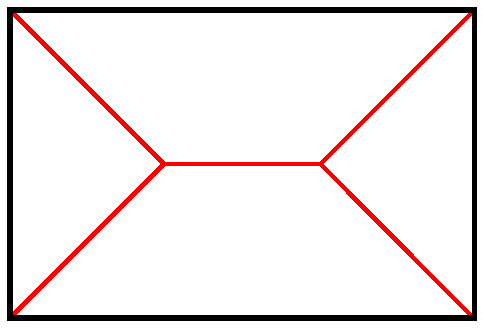
\includegraphics[width=3in]{rectangle_path}
\end{center}
\vspace{0.1in}

The extra credit is a bit tougher.
Of course, there is still a horizontal path across the middle of the island, but it is not immediately clear what the path does near the ends of the island.
It turns out that when the path approaches an end, it becomes closest to only the end, and not two points.
So the path actually stops, and doesn't reach a ``corner'' as in the rectangular case.
But where is stops is not obvious.
I can use the fact that the curvature of the ellipse is well known to identify the limits of the path.
The path stops at the point when it reaches the center of curvature of the edges.
From a quick online search, I found that the curvature $\kappa$ of an ellipse given by the formula

\[
\frac{x^{2}}{a^{2}}+\frac{y^{2}}{b^{2}}=1
\]

is defined as

\[
\kappa=\frac{ab}{\left(\sqrt{b^{2}x^{2}+a^{2}y^{2}}\right)^3}
\]

Since $a$ and $b$ are the \textit{semi}-major and \textit{semi}-minor axes, they become $a=\nicefrac{3}{2}$ and $b=1$.
The maximum curvature occurs at $y=0$, which gives $\kappa=\nicefrac{3}{2}$.
The radius of curvature $r$ is given by $r=\nicefrac{1}{\kappa}=\nicefrac{2}{3}$.
This must be removed from both sides of the major axis, so the path length in this case is $3-2(\nicefrac{2}{3})$ =
\fcolorbox{red}{white}{$\bm{{\nicefrac{5}{3}\approx1.667}}$}\,.
This can be seen in the diagram below:

\vspace{0.1in}
\begin{center}
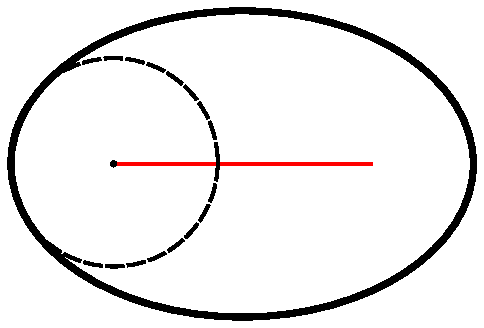
\includegraphics[width=3in]{ellipse_path}
\end{center}


\end{document}